\documentclass{article}

\usepackage{graphicx}
\usepackage{tikz}
\usepackage{tikzsymbols}
\usetikzlibrary{calc,patterns,shapes.geometric}
\pagestyle{empty}
\usepackage[margin=0pt]{geometry}
\geometry{papersize={14in,12in}}

\def\centerarc[#1](#2)(#3:#4:#5){\draw[#1] ($(#2)+({#5*cos(#3)},{#5*sin(#3)})$) arc (#3:#4:#5);}

\begin{document}
	\begin{figure}
		\centering
		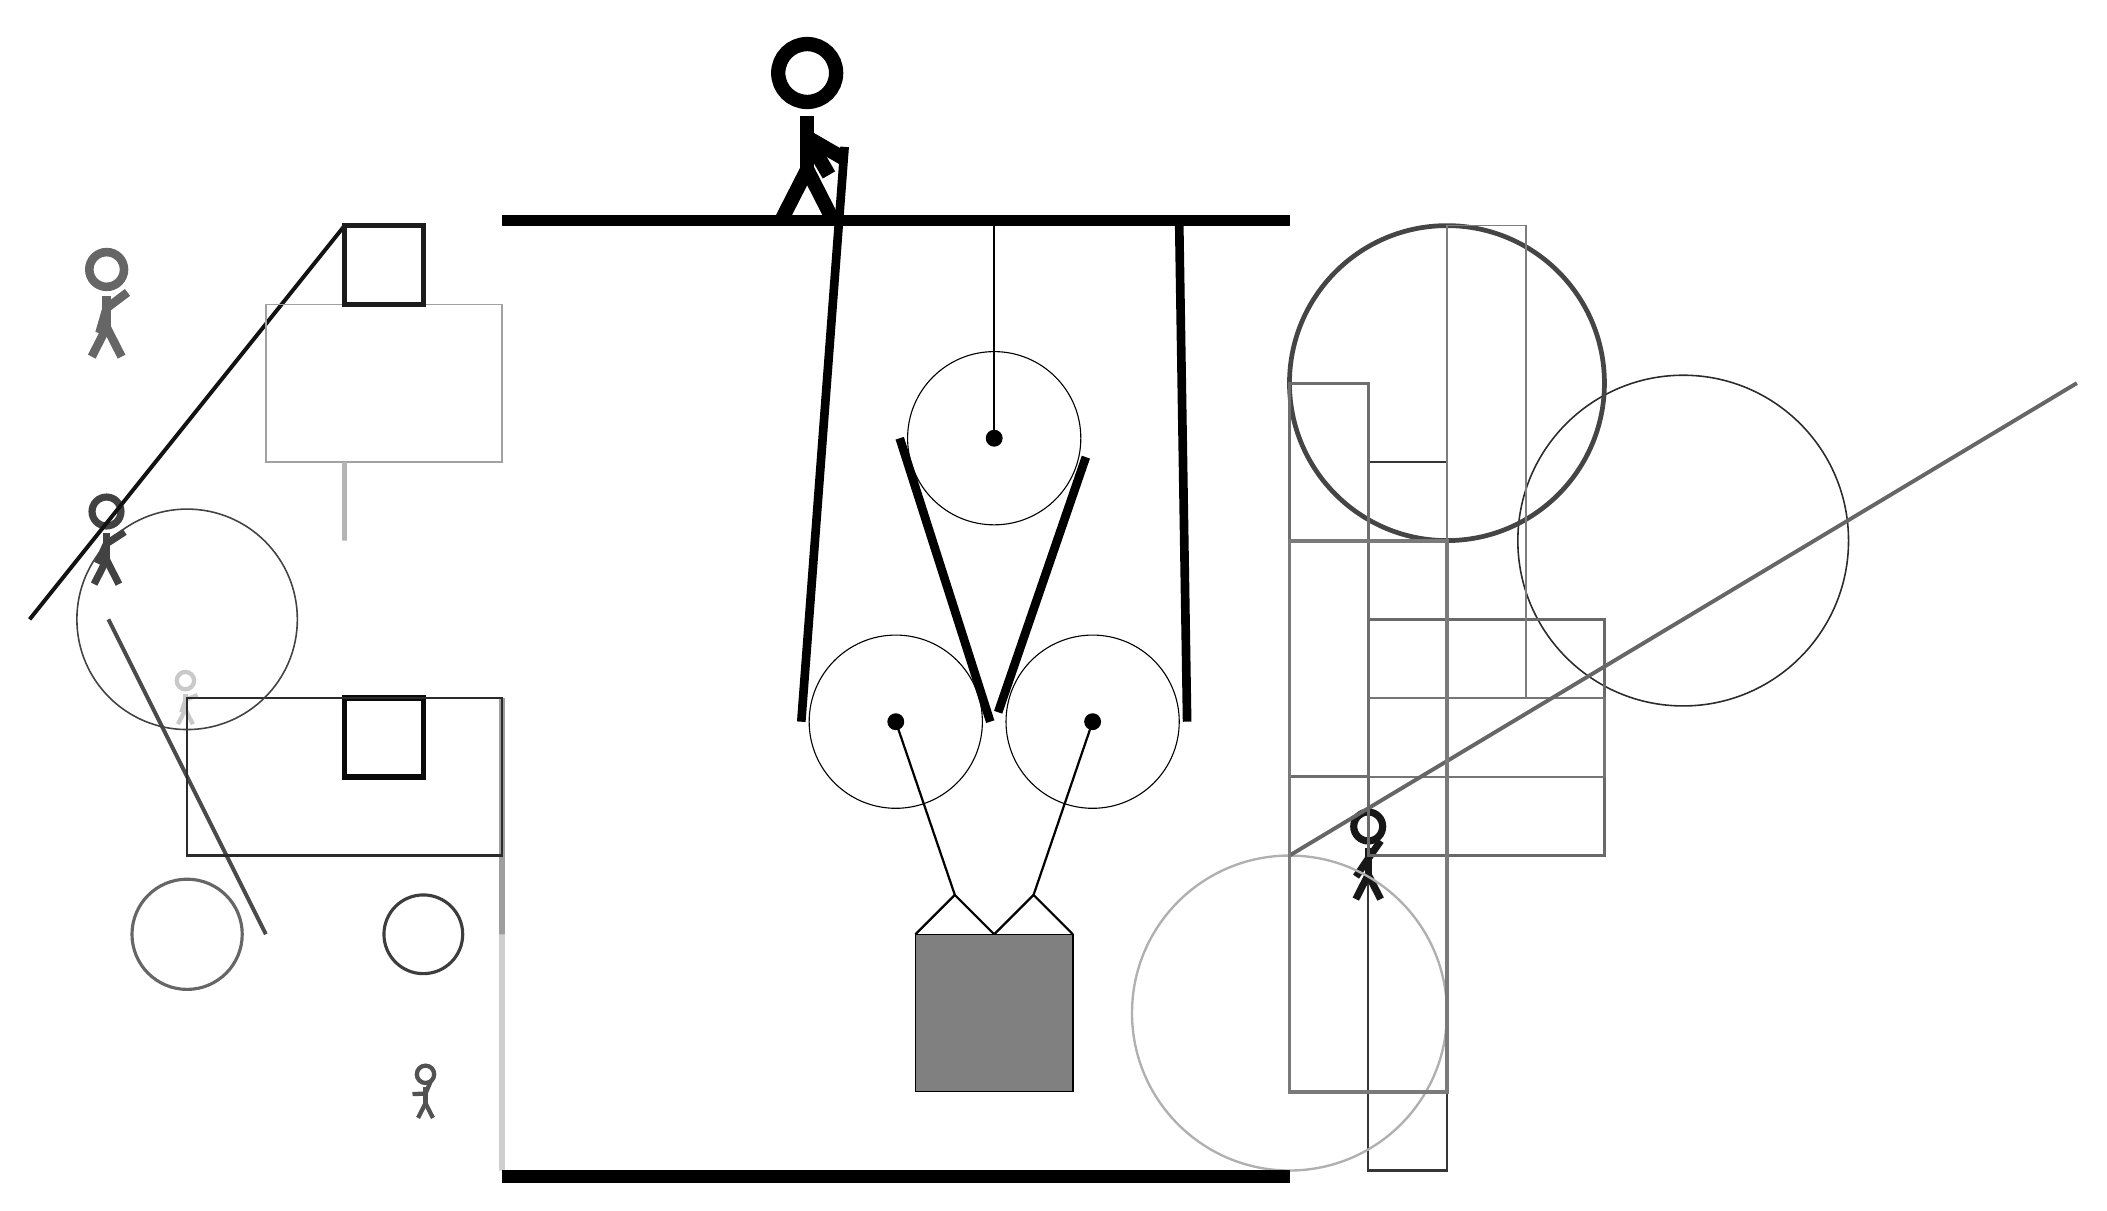
\begin{tikzpicture}
			%%%%% START %%%%%
			
			\draw[fill=black] (-4, 9) rectangle (6, 9.125);
			
			\draw (1, 2.7) circle (1.1);
			\draw[fill=black] (1, 2.7) circle (0.1);
			
			\draw [line width=0.2mm, color=black!83](11, 5) circle (2.1);
			
			\draw[line width=0.3mm, color=black!79] (8, 6) rectangle (7, -3);
			\node[line width=0.6mm, color=black!91] at (7, 1) {\Strichmaxerl[5][56][55]};
			\draw[line width=0.4mm, color=black!59] (7, 1) rectangle (10, 4);
			
			\draw [line width=0.3mm, color=black!31](6, -1) circle (2.0);
			
			\node[line width=0.3mm, color=black!74] at (-9, 5) {\Strichmaxerl[5][65][33]};
			
			\draw [line width=0.6mm, color=black!73](8, 7) circle (2.0);
			\node[line width=0.6mm, color=black!21] at (-8, 3) {\Strichmaxerl[3][72][22]};
			\draw [line width=0.4mm, color=black!76](-5, 0) circle (0.5);
			\draw [line width=0.4mm, color=black!60](-8, 0) circle (0.7);
			
			\draw[line width=0.5mm, color=black!93](-6, 9) -- (-10, 4);
			
			\draw[line width=0.2mm, color=black!51] (8, 9) rectangle (9, 3);
			\draw[line width=0.2mm, color=black!37] (-4, 8) rectangle (-7, 6);
			
			\draw[line width=0.3mm, color=black!54] (7, 3) rectangle (10, 2);
			\draw[line width=0.7mm, color=black!38] (-4, -1) rectangle (-4, 3);
			\draw[line width=0.5mm, color=black!60](6, 1) -- (16, 7);
			\node[line width=0.7mm, color=black!60] at (-9, 8) {\Strichmaxerl[6][74][37]};
			\draw[line width=0.7mm, color=black!96] (-5, 3) rectangle (-6, 2);
			\draw[line width=0.6mm, color=black!29] (-6, 6) rectangle (-6, 5);
			
			\draw[line width=0.5mm, color=black!71](-9, 4) -- (-7, 0);
			\draw[line width=0.4mm, color=black!57] (6, 2) rectangle (7, 7);
			
			\draw[line width=0.3mm, color=black!83] (-4, 1) rectangle (-8, 3);
			\draw[line width=0.7mm, color=black!19] (-4, -3) rectangle (-4, 0);
			\draw[line width=0.6mm, color=black!89] (-5, 9) rectangle (-6, 8);
			\draw[line width=0.5mm, color=black!52] (8, 5) rectangle (6, -2);
			
			\node[line width=0.2mm, color=black!68] at (-5, -2) {\Strichmaxerl[3][2][67]};
			
			\draw [line width=0.2mm, color=black!74](-8, 4) circle (1.4);
			
			\draw (2.25, 6.3) circle (1.1);
			\draw[fill=black] (2.25, 6.3) circle (0.1);
			\draw[thick] (2.25, 6.3) -- (2.25, 9);
			
			\draw (3.5, 2.7) circle (1.1);
			\draw[fill=black] (3.5, 2.7) circle (0.1);
			
			\draw[thick] (3.5, 2.7) -- (2.75, 0.5);
			\draw[thick] (1, 2.7) -- (1.75, 0.5);
			\draw[thick]  (1.25, 0) -- (1.75, 0.5) -- (2.25, 0);
			\draw[thick]  (2.25, 0) -- (2.75, 0.5) -- (3.25, 0);
			\draw[fill=black!50] (1.25, 0) rectangle (3.25, -2);
			
			\draw[line width=1.1mm] (0.35, 10) --  (-0.2, 2.7);
			\centerarc[line width=1.1mm](1, 2.7)(180:360:1.2000000000000002);
			\draw[line width=1.1mm] (2.2, 2.7) -- (1.05, 6.3);
			\centerarc[line width=1.1mm](2.25, 6.3)(-20:180:1.2000000000000002);
			\draw[line width=1.1mm](3.414, 6.06) -- (2.3, 2.82);
			\centerarc[line width=1.1mm](3.5, 2.7)(160:360:1.2000000000000002);
			\draw[line width=1.1mm](4.7, 2.7) -- (4.6, 9);
			
			\node at (-0.07, 10.2) {\Strichmaxerl[10][120][-30]};
			
			\draw[fill=black] (-4, -3) rectangle (6, -3.15);
			
			%%%%% END %%%%%
		\end{tikzpicture}
	\end{figure}	
\end{document}